\documentclass{article}

% if you need to pass options to natbib, use, e.g.:
% \PassOptionsToPackage{numbers, compress}{natbib}
% before loading nips_2016
%
% to avoid loading the natbib package, add option nonatbib:
% \usepackage[nonatbib]{nips_2016}

\usepackage[final]{nips_2016}

% to compile a camera-ready version, add the [final] option, e.g.:
% \usepackage[final]{nips_2016}

\usepackage[utf8]{inputenc} % allow utf-8 input
\usepackage[T1]{fontenc}    % use 8-bit T1 fonts
\usepackage{hyperref}       % hyperlinks
\usepackage{url}            % simple URL typesetting
\usepackage{booktabs}       % professional-quality tables
\usepackage{amsfonts}       % blackboard math symbols
%\usepackage{nicefrac}       % compact symbols for 1/2, etc.
\usepackage{microtype}      % microtypography

\usepackage{amssymb, amsmath}
\usepackage{epsfig}
\usepackage{array}
\usepackage{ifthen}
\usepackage{color}
\usepackage{fancyhdr}
\usepackage{graphicx}
\usepackage{mathtools}
\usepackage{csquotes}
\usepackage{xcolor}
\usepackage{multirow}
\newcommand\crule[3][black]{\textcolor{#1}{\rule{#2}{#3}}}

\newcommand{\tr}{\text{tr}}
\newcommand{\E}{\textbf{E}}
\newcommand{\diag}{\text{diag}}
\newcommand{\argmax}{\text{argmax}}
\newcommand{\Cov}{\text{Cov}}
\newcommand{\Var}{\text{Var}}
\newcommand{\argmin}{\text{argmin}}
\newcommand{\Vol}{\text{Vol}}
\newcommand{\comm}[1]{}
\newcommand{\indep}{\rotatebox[origin=c]{90}{$\models$}}
\newcommand{\Cor}{\text{Cor}}

\definecolor{color1}{RGB}{128,13,13}
\definecolor{color2}{RGB}{70,128,13}
\definecolor{color3}{RGB}{13,128,128}
\definecolor{color4}{RGB}{70,13,128}

\title{How many faces can be recognized? Performance extrapolation for
  multi-class classification}

% The \author macro works with any number of authors. There are two
% commands used to separate the names and addresses of multiple
% authors: \And and \AND.
%
% Using \And between authors leaves it to LaTeX to determine where to
% break the lines. Using \AND forces a line break at that point. So,
% if LaTeX puts 3 of 4 authors names on the first line, and the last
% on the second line, try using \AND instead of \And before the third
% author name.

\author{
  Charles Y.~Zheng \\
  Department of Statistics\\
  Stanford University\\
  Stanford, CA 94305 \\
  \texttt{snarles@stanford.edu} \\
  %% examples of more authors
  \And
  Rakesh ~Achanta \\
  Department of Statistics\\
  Stanford University\\
  Stanford, CA 94305 \\
  \texttt{rakesha@stanford.edu} \\
  \And
  Yuval ~Benjamini \\
  Department of Statistics \\
  Hebrew University\\
  Jerusalem, Israel\\
  \texttt{yuval.benjamini@mail.huji.ac.il}
  %% Address \\
  %% \texttt{email} \\
  %% \AND
  %% Coauthor \\
  %% Affiliation \\
  %% Address \\
  %% \texttt{email} \\
  %% \And
  %% Coauthor \\
  %% Affiliation \\
  %% Address \\
  %% \texttt{email} \\
  %% \And
  %% Coauthor \\
  %% Affiliation \\
  %% Address \\
  %% \texttt{email} \\
}

\begin{document}
% \nipsfinalcopy is no longer used

\maketitle

\begin{abstract}
The difficulty of multi-class classification generally increases with
the number of classes.  Using data from a subset of the classes, 
can we predict how well a classifier will scale with an
increased number of classes?  Under the assumption that the classes
are sampled exchangeably, and under the assumption that
the classifier is generative (e.g. QDA or Naive Bayes), we show that the expected accuracy
when the classifier is trained on $k$ classes is the $k-1$st moment
of a \emph{conditional accuracy distribution}, which can be estimated from data.
This provides the theoretical foundation for developing estimation approaches based on pseudolikelihood, 
unbiased estimation, and high-dimensional asymptotics.
We find empirically that some of the methods work well even for non-generative classifiers.
\end{abstract}

\section{Introduction}

In multi-class classification, one observes pairs $(z, y)$ where $y \in \mathcal{Y} \subset \mathbb{R}^p$ are feature vectors,
and $z$ are unknown labels, which lie in a countable label set $\mathcal{Z}$.  The goal is to construct a classification rule for
predicting the label of a new data point; generally, the classification rule $h: \mathcal{Y} \to \mathcal{Z}$
is learned from previously observed data points.  In many applications of multi-class classification,
such as face recognition or image recognition, the space of potential labels is practically infinite.
In such a setting, one might consider a sequence of classification problems on finite label subsets $\mathcal{Z}_1 \subset \cdots \subset \mathcal{Z}_K$, where in the $i$th problem, one constructs the classification rule $h^{(i)}:\mathcal{Y} \to \mathcal{Z}_i$.
Supposing that $(Z, Y)$ have a joint distribution, define the accuracy for the $i$th problem as
\[
\text{acc}^{(i)} = \Pr[h^{(i)}(Y) = Z|Z \in \mathcal{Z}_i].
\]
Using data from only $\mathcal{Z}_k$, can one predict the accuracy achieved on the larger label set $\mathcal{Z}_K$, with $K> k$?  This is the problem of \emph{prediction extrapolation}.

A practical instance of prediction extrapolation occurs in neuroimaging studies,
Kay et al. (2008) obtain fMRI brain scans which record how a single subject's visual cortex responds to natural images.
The label set $\mathcal{Z}$ corresponds to the space of all grayscale photographs of natural images,
and the set $\mathcal{Z}_1$ is a subset of 1750 photographs used in the experiment.
Kay et al. construct a classifier based on a combination of regularized multiple-response regression
and Naive Bayes: they achieve over 0.75 accuracy on the subset of 1750 photographs,
which by itself is already a convincing demonstration of the richness of the information contained in the fMRI scan.
However, it would also be of interest to know what accuracy could be achieved on a larger set of photographs.
Kay et al. calculated (based on exponential extrapolation) that it would take on the order of $10^{9.5}$ photographs
before the accuracy of the model drops below 0.10!  Directly validating this estimate would take immense resources,
so it would be useful to develop the theory needed to understand how to compute such extrapolations
in a principled way. 

However, in the fully general setting, it is impossible on construct
non-trivial bounds on the accuracy achieved on the new classes $\mathcal{Z}_K \setminus \mathcal{Z}_k$
based only on knowledge of $\mathcal{Z}_k$: after all, $\mathcal{Z}_k$ could consist entirely of well-separated classes
while the new classes $\mathcal{Z}_K \setminus \mathcal{Z}_k$ consist entirely of highly inseparable classes, or vice-versa.
Thus, the most important assumption for our theory is that of \emph{exchangeable sampling}.
The labels in $\mathcal{Z}_i$ are assumed to be an exchangeable sample from $\mathcal{Z}$.
The exchangeability further implies that the marginal distributions of $z \in \mathcal{Z}$ 
are equiprobable within every subset $\mathcal{Z}_i$. 
The condition of exchangeability ensures that the separability of random subsets of $\mathcal{Z}$ can be inferred
by looking at the empirical distributions in $\mathcal{Z}_k$, and therefore that some estimate of the achievable
accuracy on $\mathcal{Z}_K$ can be obtained.

In addition to the assumption of exchangeability, we restrict the set of classifiers considered.
We focus on \emph{generative classifiers}, which are classifiers which work by training
a model separately on each class.  This convenient property 
allows us to characterize the accuracy of the classifier by selectively conditioning on one class at a time:
in section 3, we use this technique to reveal an equivalence between 
the expected accuracies of $\mathcal{Z}_k$ to moments of a common distribution.
This moment equivalence result allows standard approaches in statistics, such as U-statistics and
nonparametric pseudolikelilood, to be directly applied to the extrapolation problem, as we discuss in section 4.
In non-generative classifiers, the classification rule has a joint dependence on the entire set of classes,
and cannot be analyzed by conditioning on individual classes.
Nevertheless, in Section 5, we see that our methods achieve similarly accurate extrapolation for both
generative and non-generative classifiers in real data examples.

\section{Setting}

Having motivated the problem of prediction extrapolation,
we now reformulate the problem for notational and theoretical convenience.
Instead of requiring $\mathcal{Z}_k$ to be a random subset of $\mathcal{Z}$ as we did in section 1, take
$\mathcal{Z}=\mathbb{N}$ and $\mathcal{Z}_k = \{1,\hdots, k\}$.
We fix the size of $\mathcal{Z}_k$ without losing generality, since any monotonic sequence of 
finite subsets can be embedded in a sequence with $|\mathcal{Z}_k| = k$.
In addition, rather than randomizing the labels, we will randomize the marginal distribution of each label;
Towards that end, let $\mathcal{Y} \subset \mathbb{R}^p$ be a space of feature vectors, and
let $\mathcal{P}(\mathcal{Y})$ be a measurable space of probability distributions on $\mathcal{Y}$.
Let $\mathcal{F}$ be a probability measure on $\mathcal{P}$,
and let $F_1, F_2,\hdots$ be an infinite sequence of i.i.d. draws from $\mathbb{F}$.
We refer to $\mathbb{F}$, a probability measure on probability measures, as a \emph{meta-distribution}.
The distributions $F_1,\hdots, F_k$ are the marginal distributions of the first $k$ classes.
We therefore rewrite the accuracy as
\[
\text{acc}^{(i)} = \frac{1}{t}\sum_{i=1}^t \Pr_{F_i}[h^{(t)}(Y) = i].
\]
where the probabilities are taken over $Y \sim F_i$.

In order to construct the classification rule $h^{(t)}$, we need data from the classes $F_1,\hdots, F_t$.
In most instances of multi-class classification, one observes independent observations from each $F_i$
which are used to construct the classifier.  Since the order of the observations
does not generally matter, a sufficient statistic for the training data for the $t$th classification problem
is the collection of empirical distributions
$\hat{F}_1^{(t)},\hdots,\hat{F}_t^{(t)}$ for each class.
Henceforth, we make the simplifying assumption that the training data for the $i$th class remains fixed
from $t =i, i+1,\hdots$, so we drop the superscript on $\hat{F}_i^{(t)}$.
Write $\hat{\mathbb{F}}(F)$ for the conditional distribution of $\hat{F}_i$ given  $F_i = F$;
also write $\hat{\mathbb{F}}$ for the marginal distribution of $\hat{F}$ when $F \sim \mathbb{F}.$
As an example, suppose every class has the number of training examples $r \in \mathbb{N}$; then $\hat{F}$
is the empirical distribution of $r$ i.i.d. observations from $F$, and $\hat{\mathbb{F}}(F)$ is the \emph{empirical meta-distribution} of $\hat{F}$.
Meanwhile, $\hat{\mathbb{F}}$ is the meta-distribution of the empirical distribution of $r$ i.i.d. draws from a random $F \sim \mathbb{F}$.


\subsection{Multi-class classification}

Extending the formalism of Tewari and Bartlett (2007),
we define a classifier as a collection of mappings
$\mathcal{M}_i: \mathcal{P}(\mathcal{Y})^k \times \mathcal{Y} \to \mathbb{R}$ called \emph{margin functions.}
Intuitively speaking, each margin function \emph{learns a model} from the first $k$ arguments, which are
the empirical marginals of the $k$ classes, which it uses to assign a \emph{margin} or \emph{score} to the
\emph{query point} $y \in \mathcal{Y}$.  A higher score $\mathcal{M}_i(\hat{F}_1,\hdots, \hat{F}_k, y)$ indicates a higher estimated probability that $y$ belongs to the $k$th class.  
Therefore, the classification rule corresponding to a classifier $\mathcal{M}_i$ assigns
a class with maximum margin to $y$:
\[
h(y) = \argmax_{i \in \{1,\hdots, k\}} \mathcal{M}_i(y).
\]
For some classifiers, the margin function $\mathcal{M}_i$ is especially simple
in that $\mathcal{M}_i$ is only a function of $\hat{F}_i$ and $y$.
Furthermore, due to symmetry, in such cases one can write
\[
\mathcal{M}_i(\hat{F}_1,\hdots, \hat{F}_k, y) = \mathcal{Q}(\hat{F}_i, y)
\]
where $\mathcal{Q}$ is called a \emph{single-class margin} (or simply \emph{margin}.)
For notational convenience, we assume that ties occur with probability
zero: that is, $\hat{\mathbb{F}}$ and $\mathcal{Q}$ jointly satisfy the
\emph{tie-breaking} property:
\begin{equation}\label{eq:tie}
\Pr[\mathcal{Q}(\hat{F}, y) = \mathcal{Q}(\hat{F}', y)] = 0.
\end{equation}
for all $y \in \mathcal{Y}$, where $\mathbb{F}, \mathbb{F}' \stackrel{iid}{\sim} \hat{\mathbb{F}}$.
Quadratic discriminant analysis and Naive Bayes are two examples of
generative classifiers.  For QDA, the margin is given by
\[
\mathcal{Q}_{QDA}(\hat{F}, y) = -(y - \mu(\hat{F}))^T \Sigma(\hat{F})^{-1} (y-\mu(\hat{F})) - \log\det(\Sigma(\hat{F}))
\]
where $\mu(F) = \int y dF(y)$ and $\Sigma(F) = \int (y-\mu(F))(y-\mu(F))^T dF(y)$.
In Naive Bayes, the margin is
\[
\mathcal{Q}_{NB}(\hat{F},  y) = \sum_{i=1}^n \log \hat{f}_i(y_i)
\]
where $\hat{f}_i$ is a density estimate for the $i$th component of
$\hat{F}$.
The \emph{generative} property allows us to prove strong results about the accuracy of the classifier
under the exchangeable sampling assumption, as we see in Section 3.

\section{Prediction extrapolation for generative classifiers}

Let us specialize to the case of a generative classifier, with scoring rule $\mathcal{Q}$.
Consider estimating the expected accuracy at time $t$, \[p_t
\stackrel{def}{=} \E[\text{acc}^{(t)}].\]
Define the \emph{conditional accuracy} function $u(\hat{F}, y)$ which maps a
distribution $\hat{F}$ on $\mathcal{Y}$ and a \emph{test} observation $y$ to
a real number in $[0,1]$.  The conditional accuracy gives the
probability that for independently drawn $\hat{F}'$ from $\hat{\mathbb{F}}$, that
$\mathcal{Q}(\hat{F}, y)$ will be greater than $\mathcal{Q}(\hat{F}', y)$:
\[
u(\hat{F}, y) = \Pr_{\hat{F} \sim \hat{\mathbb{F}}}[\mathcal{Q}(\hat{F}, y) > \mathcal{Q}(\hat{F}', y)].
\]
Define the \emph{conditional accuracy} distribution $\nu$ as the law
of $u(\hat{F}, Y)$ where $\hat{F}$ and $Y$ are generated as follows:
(i) a true distribution $F$ is drawn from $\mathbb{F}$; (ii) the query $Y$ is drawn from $F$, 
and (iii) the empirical distribution $\hat{F}$ is drawn from $\hat{\mathbb{F}}(F)$ 
(e.g., the distribution of the empirical distribution of $r$ i.i.d. observations drawn from $F$),
with $Y$ independent of $\hat{F}$.  The significance of the conditional accuracy
distribution is that the expected generalization error $p_t$ can be
written in terms of its moments.

\noindent\textbf{Theorem 3.1.} \emph{
Let $\mathcal{Q}$ be a single-distribution margin, and let $\mathbb{F}$, $\hat{F}(F)$ be a distribution on $\mathcal{P}(\mathcal{Y}).$
Let $U$ be defined as the random variable
\[
U = u(\hat{F}, Y)
\]
for $F \sim \mathbb{F}$, $Y \sim F$, and $\hat{F} \sim \hat{\mathbb{F}}(F)$ with $Y \perp \hat{F}$.
Recall the definition
\[
p_k = \E[acc^{(k)}] = \E\left[\frac{1}{t}\sum_{i=1}^k \Pr_{Y \sim F_i}[\mathcal{Q}(\hat{F}_i, Y) > \max_{j \neq i}\mathcal{Q}(\hat{F}_j, Y)]\right].
\]
Then \[p_k = \E[U^{k-1}].\]
}

\noindent\textbf{Proof.}  
Write $q^{(i)}(y) = \mathcal{Q}(\hat{F}_i, y)$.
By using conditioning and
conditional independence, $p_k$ can be written
\begin{align*}
p_k &= \E\left[ \frac{1}{k}\sum_{i=1}^k  \Pr_{F_i}[q^{(i)}(Y) > \max_{j\neq i} q^{(j)}(Y)] \right]
\\&= \E\left[ \Pr_{F_1}[q^{(1)}(Y) > \max_{j\neq 1} q^{(j)}(Y)] \right]
\\&= \E_{F_1}[\Pr[q^{(1)}(Y) > \max_{j\neq 1} q^{(j)}(Y)|\hat{F}_1, Y]]
\\&= \E_{F_1}[\Pr[\cap_{j > 1} q^{(1)}(Y) > q^{(j)}(Y)|\hat{F}_1, Y]]
\\&= \E_{F_1}[\prod_{j > 1}\Pr[q^{(1)}(Y) > q^{(j)}(Y)|\hat{F}_1, Y]]
\\&= \E_{F_1}[\Pr[q^{(1)}(Y) > q^{(2)}(Y)|\hat{F}_1, Y]^{k-1}]
\\&= \E_{F_1}[u(\hat{F}_1, Y)^{k-1}] = \E[U^{k-1}].
\end{align*}
$\Box$

Theorem 3.1 tells us that the problem of extrapolation can be
approached by attempting to estimate the conditional accuracy
distribution.  The $(t-1)$th moment of $U$ gives us $p_t$, which will
in turn be a good estimate of $\text{acc}^{(t)}$.

While $U = u(\hat{F}, Y)$ is not directly observed, we can obtain unbiased estimates of $u(\hat{F}_i, y)$
by using test data.  For any $\hat{F}_1,\hdots, \hat{F}_k$, and independent test point $Y \sim F_i$, define
\begin{equation}\label{eq:hatu}
\hat{u}(\hat{F}_i, Y) = \frac{1}{k -1}\sum_{j \neq i} I(\mathcal{Q}(\hat{F}_i, Y) > \mathcal{Q}(\hat{F}_j, Y)).
\end{equation}
Then $\hat{u}(\hat{F}_i, Y)$ is an unbiased estimate of $u(\hat{F}_i, Y)$, as stated in the following theorem.

\noindent\textbf{Theorem 3.2.}\emph{
Assume the conditions of theorem 3.1.
Then defining 
\begin{equation}\label{eq:veq}
V = (k-1)\hat{u}(\hat{F}_i, y),\end{equation}
we have
\[V \sim \text{\emph{Binomial}}(k, u(\hat{F}_i, y)).\]
Hence,
\[\E[\hat{u}(\hat{F}_i, y)] = u(\hat{F}_i, y).\]
}

In section 4, we will use this result to estimate the moments of $U$.
Meanwhile, since $U$ is a random variable on $[0, 1]$, we also conclude that $p_t$ follows a \emph{mixed exponential decay}.
Let $\alpha$ be the law of $-\log(U)$.
Then from change-of-variables $\kappa =-\log(u)$, we get
\[\E[\text{acc}^{(t)}] = \E[U^{t-1}] = 
\int_0^1 u^{t-1} d\nu(u) = \int_0^1 e^{t\log(u)} \frac{1}{u}d\nu(u) = 
\int_{\mathbb{R}^{+}} e^{-\kappa t} d\alpha(\kappa).\]
This fact immediately suggests the technique of fitting an mixture of exponentials to the test error at $t =2,3,\hdots, k$:
we explore this idea further in Section 4.1.

\subsection{Properties of the conditional accuracy distribution}

The conditional error distribution $\nu$ is determined by $\mathbb{F}$
and $\mathcal{Q}$.  What can we say about the the conditional accuracy
distribution without making any assumptions on either $\mathbb{F}$ or
$\mathcal{Q}$?  The answer is: not much--for an arbitrary probability
measure $\nu'$ on $[0,1]$, one can construct $\mathbb{F}$ and
$\mathcal{Q}$ such that $\nu = \nu'$, even if one makes the \emph{perfect sampling assumption} that $\hat{F}=F.$

\noindent\textbf{Theorem 3.3.} \emph{ Let $U$ be defined as in Theorem
  3.1, and let $\nu$ denote the law of $U$.  Then, for any probability
  distribution $\nu'$ on $[0,1]$, one can construct a
  meta-distribution $\mathbb{F}$ and a scoring rule $\mathcal{Q}$ such
  that $\nu = \nu'$ under perfect sampling (that is, $\hat{F} = F$.)  }

\textbf{Proof.}  
Let $G$ be the cdf of $\nu$, $G(x) = \int_0^x d\nu(x)$, and let $H(u) = \sup_x \{G(x) \leq u\}$.
Define $\mathcal{Q}$ by
\[
\mathcal{Q}(\hat{F}, y) = \begin{cases}
0 &\text{ if }\mu(\hat{F}) > y + H(y)\\
0 & \text{ if }y + H(y) > 1 \text{ and }\mu(\hat{F}) \in [H(y) - y, y]\\
1 + \mu(\hat{F}) - y &\text{ if } \mu(\hat{F}) \in [y, y + H(y)]\\
1 + y + \mu(\hat{F}) &\text{ if }\mu(\hat{F}) + H(y) > 1 \text{ and }\mu(\hat{F}) \in [0, H(y) - y]. 
\end{cases}
\]
Let $\theta \sim \text{Uniform}[0,1]$,
and define $F \sim \mathbb{F}$ by $F = \delta_\theta$, and also $\hat{F} = F.$
A straightforward calculation yields that $\nu = \nu'$. $\Box$

On the other hand, we can obtain a positive result if we assume that
the classifier approximates a \emph{Bayes classifier.}
Assuming that $F$ is absolutely continuous with respect to Lebesgue measure $\Lambda$ with probability one,
a Bayes classifier results from assuming perfect sampling ($\hat{F} = F$) and taking
$\mathcal{Q}(\hat{F}, y) = \frac{dF}{d\Lambda}(y)$.
Theorem 3.4. states that for a Bayes classifier, $\nu$ has a density $\eta(u)$ which is monotonically increasing.
Since a `good' classifier approximates the Bayes classifier, we intuitively expect that a monotonically
increasing density $\eta$ is a good model for the conditional accuracy distribution of a `good' classifier.

\noindent\textbf{Theorem 3.4.} \emph{ Assume the conditions of theorem 3.1, and further suppose
that $\hat{F} = F$, $F$ is absolutely continuous with respect to $\Lambda$ with probability one,
and that $\mathcal{Q}(\hat{F}, y) = \frac{dF}{d\Lambda}(y)$.
Let $\nu$ denote the law of $U$.    Then $\nu$ has a density $\eta(u)$ on $[0, 1]$ which is monotonic in $u$.
}

\noindent\textbf{Proof.}
It suffices to prove that
\[
\nu([u, u + \delta]) < \nu([v, v + \delta])
\]
for all $0 < u < v < 1$ and $0 < \delta < 1-v$.
Let $\mathcal{P}_{ac}(\mathcal{Y})$ denote the space of distributions supported on $\mathcal{Y}$ which are
absolutely continuous with respect to $p$-dimensional Lebesgue measure $\Lambda$.
For $F \in \mathcal{P}_{ac}(\mathcal{Y})$, let $f = \frac{dF}{d\Lambda}$. Define the set 
\[
J_F(A) =\{y \in \mathcal{Y}: u(F, y) \in A\} = \left\{y \in \mathcal{Y}: \Pr_{Y \sim F}[f(y) > f(Y)] \in A\right\}.
\]
for all $A \subset [0, 1].$
One can verify that for all $F \in \mathcal{P}_{ac}\mathcal{Y}$,
\[
F(J_F([u, u + \delta])) \leq F(J_F([v, v + \delta])).
\]
Yet, since
\[
\Pr[U \in [u, u + \delta]] = \Pr_{F \sim \mathbb{F}}[Y \in J_F([u, u + \delta])] = \E_{F \sim \mathbb{F}}[F(J_F([u, u + \delta]))]
\]
\[
\Pr[U \in [v, v + \delta]] = \Pr_{F \sim \mathbb{F}}[Y \in J_F([v, v + \delta])] = \E_{F \sim \mathbb{F}}[F(J_F([v, v + \delta]))]
\]
we obtain
\[
\Pr[U \in [u-\delta, u + \delta]] \leq \Pr[U \in [v - \delta, v + \delta]].
\]
Taking $\delta \to 0$, we conclude the theorem. $\Box$\newline

\section{Estimation}

Suppose we have $m$ independent test repeats per class, $y^{(i),1}\hdots, y^{(i), m}$.
Let us define
\[
V_{i,j} = \sum_{\ell\neq i} I(\mathcal{M}_i(\hat{F}_1,\hdots, \hat{F}_k, y^{(i, j)})  > \mathcal{M}_\ell(\hat{F}_1,\hdots, \hat{F}_k, y^{(i, j)})),
\]
which coincides with the definition \eqref{eq:veq} in the special case that $\mathcal{M}$ is generative.

At a high level, we have a hierarchical model where $U$ is drawn from a distribution $nu$ on $[0, 1]$
and then $V_{i, j} \sim \text{Binomial}(k, U)$;

Let us assume that $U$ has a density $\eta(u)$: then the marginal distribution of $V_{i, j}$ can be written
\[
\Pr[V_{i,j} = \ell] = \begin{pmatrix}
k \\ \ell
\end{pmatrix}
\int_0^1 u^\ell (1-u)^{k-\ell} \eta(u) du.
\]
However, the observed $\{V_{i, j}\}$ do \emph{not} comprise an i.i.d. sample.

We discuss the following three approaches for estimating $p_t =
\E[U^{t-1}]$ based on $V_{i, j}$.  The first is an extension of \emph{unbiased
  estimation} based on binomial U-statistics, which is discussed in
Section 4.1.  The second is the \emph{pseudolikelihood} approach.  In
problems where the marginal distributions are known, but the
dependence structure between variables is unknown, the
\emph{pseudolikelihood} is defined as the product of the marginal
distributions.  For certain problems in time series analysis and
spatial statistics, the maximum psuedolikelihood estimator (MPLE) is
proved to be consistent (Arnold 1991).  We discuss psuedolikelihood-based
approaches in Section 4.2.  Thirdly, we note that the high-dimensional
theory of Anon 2006 can be applied for prediction accuracy, which we discuss in Section 4.3.

\subsection{Extensions of unbiased estimation}

If $V \sim \text{Binomial}(k, U)$, then an unbiased estimator of $U^t$ exists
if and only if $0 \leq t \leq k$.

The theory of U-statistics provides the minimal variance unbiased estimator for $U^t$:
\[
U^t = \E\left[\begin{pmatrix}
V \\ t
\end{pmatrix}
\begin{pmatrix}
k \\ t
\end{pmatrix}^{-1}\right].
\]

This result can be immediately applied to yield an unbiased estimator of $p_t$, when $t \leq k$:
\begin{equation}\label{eq:ustat}
\hat{p}_t^{UN} =  \frac{1}{km}\sum_{i=1}^k\sum_{j=1}^{m} \begin{pmatrix}
V_{i, j} \\ t-1
\end{pmatrix}
\begin{pmatrix}
k \\ t-1
\end{pmatrix}^{-1}.
\end{equation}
However, since $\hat{p}_t^{UN}$ is undefined for $k \geq t$, we can use exponential extrapolation
to define an extended estimator $\hat{p}_t^{EXP}$ for $k > t$.
Let $\hat{\alpha}$ be a measure defined by solving the optimization problem
\[
\text{minimize} \sum_{t=2}^{k} \left(\hat{p}_t^{UN} - \int_0^\infty \exp[-t\kappa] d\alpha(\kappa)\right)^2
\]
After discretizing the measure $\hat{\alpha}$, we obtain a convex optimization problem
which can be solved using non-negative least squares (Lawson 1974).
Then define
\[
\hat{p}_t^{EXP} = \begin{cases}
\hat{p}_t^{UN}&\text{ for }t \leq k,\\
\int_0^\infty \exp[-t\kappa] d\hat{\alpha}(\kappa))&\text{ for }t > k.
\end{cases}
\]

\subsection{Maximum pseudolikelihood}

The pseudolikelihood is defined as
\begin{equation}\label{eq:psuedo}
\ell(\eta) = \sum_{i=1}^k \sum_{j=1}^{m} \log\left(\int u^{V_{i, j}} (1-u)^{k - V_{i, j}} \eta(u) du\right),
\end{equation}
and a maximum pseudolikelihood estimator (MPLE) is defined as any
density $\hat{\eta}$ such that
\[
\ell(\hat{\eta}_{MPLE}) = \sup_{\eta} \ell(\eta).
\]
The motivation for $\hat{\eta}_{MPLE}$ is that it consistently
estimates $\eta$ in the limit where $k \to \infty$.
However, in finite samples, $\hat{\eta}_{MPLE}$ is not uniquely defined,
and if we define the plug-in estimator
\[
\hat{p}_t^{MPLE} = \int u^{t-1} \hat{\eta}_{MPLE}(u) du,
\]
$\hat{p}_t^{MPLE}$ can vary over a large range, depending on which $\hat{\eta} \in \argmax_{\eta} \ell_t(\eta)$
is selected.
These shortcomings motivate the adoption of additional constraints on the estimator $\hat{\eta}.$

Theorem 3.4. motivates the \emph{monotonicity constraint} that $\frac{d\hat{\eta}}{du} > 0$.
A second constraint is to restrict the $k$th moment of $\hat{\eta}$ to match the unbiased estimate.
The addition of these constraints yields the constrained PMLE
$\hat{\eta}_{CON}$, which is obtained by solving
\[
\text{maximize }\ell(\eta) \text{ subject to }\int u^{k-1} \eta(u) du = \hat{p}_k^{UN}\text{ and }\frac{d\hat{\eta}}{du} > 0.
\]
By discretizing $\eta$, all of the above maximization problems can be solved using a general-purpose convex solver\footnote{
We found that the CVX discipline convex programming language, using the ECOS second-order cone programming solver,
succeeds in optimizing the problems where the dimension of the discretized $\eta$ is as large as 10,000 (Hong 2014, Domahidi 2013.)}.

\subsection{High-dimensional asymptotics}

Under a number of conditions on the distribution $\mathbb{F}$, including (but not limited to) having a large dimension $p$,
Anon 2016 relate the accuracy $p_t$ of the Bayes classifier to the mutual information between the label $z$ and
the response $y$:
\[
p_t = 1-\pi_t(\sqrt{2I(Z; Y)}).
\]
where
\[
\pi_k = \pi_k(c) = 1 - \int_{\mathbb{R}} \phi(z - c)  \Phi(z)^{k-1} dz.
\]
While our goal is not to estimate the mutual information, we note that the results of Anon 2016
imply a relationship between $p_k$ and $p_K$ for the Bayes error under the high-dimensional regime:
\[
p_K = 1-\pi_K\left(\frac{1}{2}(\pi_k^{-1}(1-p_k))^2\right).
\]
Therefore, under the high-dimensional conditions of Anon 2016 and assuming that the classifier approximates
the Bayes classifier, we naturally obtain the following estimator
\[
\hat{p}_t^{HD} = 1-\pi_K\left(\frac{1}{2}(\pi_k^{-1}(1-\hat{p}_k^{UN}))^2\right).
\]

\section{Results}

We applied the methods described in Section 4 to predict the 400-class accuracy of multinomial
logistic regression, SVM, and $\epsilon$-nearest neighbors\footnote{$k$-nearest neighbors with $k = \epsilon n$ for fixed $\epsilon > 0$} on a Telegu character classification task,
using 20-class data with 100 examples per class.  The results are displayed in Figure 1.
The constrained PMLE method performs best, obtaining the best accuracy for two out of the three classifiers.

\begin{figure}
\centering
\begin{tabular}{|c||c|c|c|c|}\hline
Classifier & Ground truth & $\hat{p}^{(EXP)}$ & $\hat{p}^{(CON)}$ & $\hat{p}^{(HD)}$\\ \hline
Logistic & 0.711 & 0.844 & \textbf{0.721} & 0.686 \\ \hline
SVM & 0.545 & 0.737 & 0.575 & \textbf{0.546} \\ \hline
$\epsilon$-NN & 0.591 & 0.903 & \textbf{0.608} & 0.839\\ \hline
\end{tabular}
\caption{Prediction extrapolation: predicting the error on 400 classes using data from 20 classes on a Telugu character dataset.
$\epsilon = 0.002$ for $\epsilon$-nearest neighbors.}
\end{figure}


%\begin{figure}
%\centering
%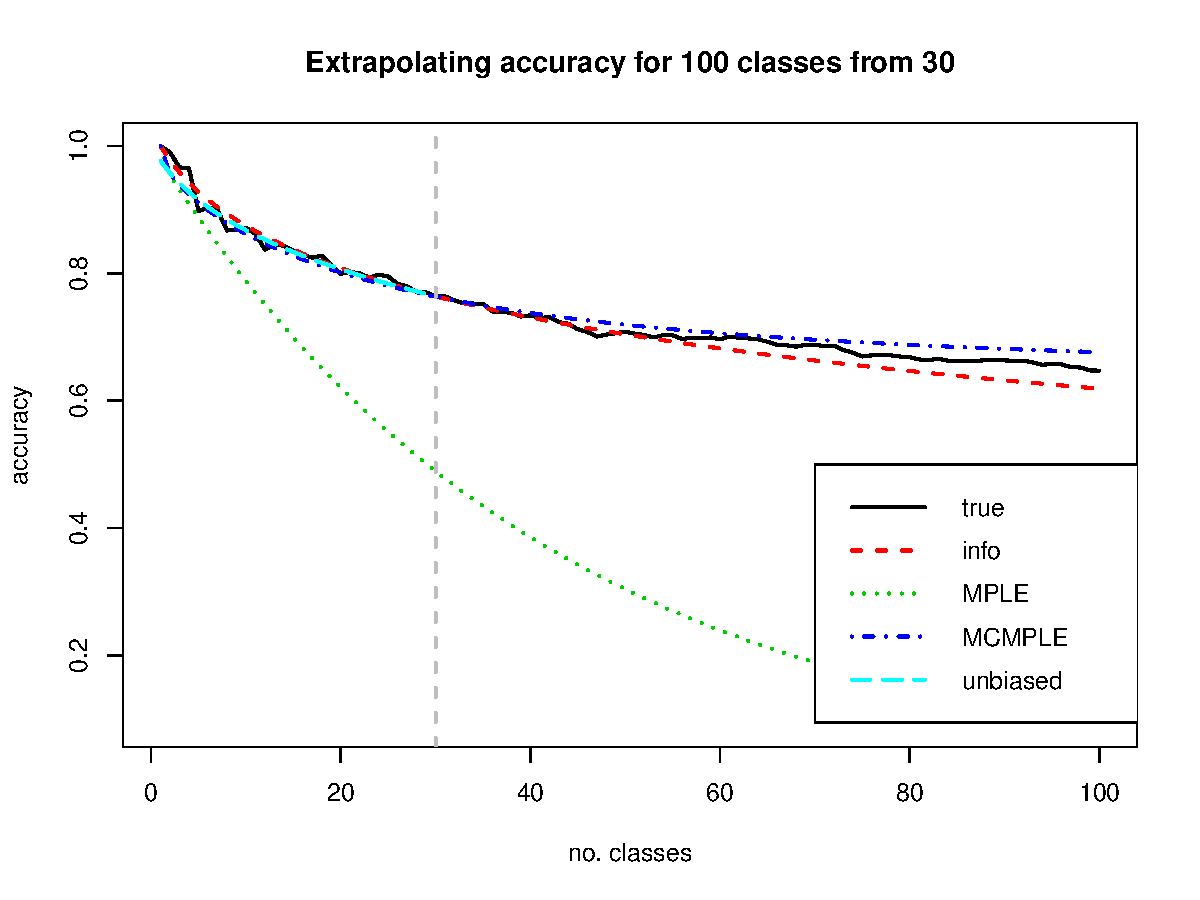
\includegraphics[scale = 0.6]{cifar_example.pdf}
%\caption{Extrapolation classification performance for CIFAR data.  (This simulation needs to be fixed later.)
%PMLE: maximum psuedolikelihood. MCPMLE: Moment-constrained max psuedolikelihood.  Info: Zheng and Benjamini's info-%theoretic method.
%Unbiased: U-statistic (cannot be used to extrapolate.) }
%\end{figure}

\section{Discussion}

We have developed a theory of prediction extrapolation for generative classifiers,
under the assumption of exchangeable classes.  However, empirical results indicate
that our methods generalize beyond generative classifiers.
A possible explanation is that many non-generative classifiers are \emph{asymptotically generative},
meaning that $\mathcal{M}_i^{(t)}$, the $i$th margin for the $t$th classification problem in the sequence,
converges to a function of $\hat{F}_i$ and $y$ with probability one:
\begin{equation}\label{eq:agen}
\lim_{t \to \infty} \mathcal{M}_i^{(t)}(\hat{F}_1,\hdots, \hat{F}_t, y) = \mathcal{Q}(\hat{F}_i, y) \text{ w.h.p. }
\end{equation}
While asymptotically generative classifiers can be decomposed in a similar manner as generative classifiers,
they need not share the same practical \emph{limitations} as generative classifiers.
A generative classifier requires the user to specify the scoring function $\mathcal{Q}$ in advance:
this practically requires some prior knowledge about the marginal distributions of the classes,
e.g. that the marginal distributions are approximately multivariate Gaussian.
But the scoring function $\mathcal{Q}$ appearing in the definition of an asymptotically generative classifier
\emph{need not be specified} by the user: 
it can (and usually does) depend on the unknown meta-distribution $\mathbb{F}$.
One can show that one-vs-one, one-vs-all, and $\epsilon$-nearest neighbors satisfy the definition \eqref{eq:agen}
after assuming some additional continuity conditions; however, the definition \eqref{eq:agen} does not
suffice to extend the key result in theorem 3.1.  Finding appropriate conditions to obtain a useful
definition of an \emph{asymptotically generative} classifier is the subject of current work.

The assumption of exchangeability greatly limits the scope of application for our methods.
 Many multi-class classification problems
have a hierarchical structure, where the initial label set $\mathcal{Z}_1$ corresponds to a coarse-grained partition of the instances, and an expanded label set $\mathcal{Z}_2$ corresponds to a refinement of the partition induced by $\mathcal{Z}_1$:
for instance, $\mathcal{Z}_1$ consists of the categories $\{\text{animal}, \text{vegetable}, \text{mineral}\}$,
while $\mathcal{Z}_2$ consists of subcategories 
$\{\text{mammal}, \text{bird}, \text{insect}, \text{reptile}, \text{fungus}, \text{tree}, \text{flower}, \text{rock}, \text{metal}\}$.
Not only is $\mathcal{Z}_2$ not a superset of $\mathcal{Z}_1$, but the marginal distributions within $\mathcal{Z}_2$ are necessarily more concentrated than the marginals of $\mathcal{Z}_1$.
Many non-hierarchical classification problems are also excluded by the requirement of exchangeability.
Consider the problem of annotating spoken words: the set $\mathcal{Z}_1$ might consist of data from the 100 most common words, while the set $\mathcal{Z}_2$ consists of data from the 1000 most common words.
Exchangeability is violated because the words $z \in \mathcal{Z}$ are not equiprobable, but rather follow a long-tail law.
It would be interesting to extend our theory to the hierarchical setting, or to handle non-hierarchical settings
with non-uniform prior class probabilities, but again we leave the subject for future work.

\subsubsection*{Acknowledgments}

CZ is supported by an NSF graduate research fellowship.

\section*{References}

\small

[X] Ng, Andrew Y., and Michael I. Jordan. "On Discriminative vs. Generative classifiers: A comparison of logistic regression and naive Bayes." (2002).

[X] Arnold, Barry C., and David Strauss. ``Pseudolikelihood estimation: some examples." Sankhya: The Indian Journal of Statistics, Series B (1991): 233-243.

[X] Lawson, Charles L., and Richard J. Hanson. Solving least squares problems. Vol. 161. Englewood Cliffs, NJ: Prentice-hall, 1974.

[X] Hong, Jenny, Karanveer Mohan, and David Zeng. ``CVX. jl: A Convex Modeling Environment in Julia." (2014).

[X] Domahidi, Alexander, Eric Chu, and Stephen Boyd. "ECOS: An SOCP solver for embedded systems." Control Conference (ECC), 2013 European. IEEE, 2013.

[X] Naselaris, T., Kay, K. N., Nishimoto, S., \& Gallant,
J. L. (2011). Encoding and decoding in fMRI. \emph{Neuroimage}, 56(2),
400-410.

[X] Friedman, Jerome, Trevor Hastie, and Robert Tibshirani. \emph{The elements
of statistical learning.} Vol. 1. Springer, Berlin: Springer series in
statistics, 2008.

\end{document}









Ideally, we could extend Theorem 2.2 for asymptotic generative classifiers, but a stronger condition is needed.
Note that under the tie-breaking assumption, one can always take $\mathcal{Q}$ in \eqref{eq:agen} so that
\[
\Pr[\mathcal{Q}(\hat{F}, y) < u] = u\text{ for }u \in [0,1],
\]
for all $y \in \mathcal{Y}$: we refer to such $\mathcal{Q}$ as \emph{calibrated.}
We define a \emph{uniformly asymptotic generative} classifier by adding conditions on the worst-case rate that
$\mathcal{M}_i$ converges to calibrated $\mathcal{Q}$: these additional conditions are sufficient for the generalization of Theorem 2.3.  We now give the definition and the theorem.

\textbf{Definition 2.1.}  \emph{(Uniformly asymptotically generative) Suppose classifier $\mathcal{M}$ satisfies \eqref{eq:agen} for calibrated $\mathcal{Q}$, and furthermore that
\[
\lim_{t \to \infty} \sup_{i \leq t} \frac{1}{t}\sum_{j=1}^t \Pr_{F_j}[\mathcal{M}(\hat{F}_1,\hdots, \hat{F}_t, Y) - \mathcal{Q}(\hat{F}_i, Y)| > \epsilon] \to 0
\]
with probability one for all $\epsilon > 0$.  Then we say that $\mathcal{M}$ is uniformly asymptotically generative.}

\textbf{Theorem 2.3}\emph{
Let $\mathcal{Q}$ be the scoring function of a uniformly generative classifier, and 
assume that $F_1,\hdots, F_k \stackrel{iid}{\sim} \mathbb{F}$ and $\hat{F}_i \sim \hat{\mathbb{F}}(F_i)$ independently,
following the notation of section 2.
Further assume that $\mathcal{Q}$ and $\mathbb{F}$ satisfy the tie-breaking property \eqref{eq:tie}.
Then, recalling the definition of accuracy,
\[
\text{acc}^{(t)} = \frac{1}{t}\sum_{i=1}^t \Pr_{Y \sim F_i}[\mathcal{M}_i(\hat{F}_1,\hdots,\hat{F}_t, Y) > \argmax_{i > j} \mathcal{M}_j(\hat{F}_1,\hdots, \hat{F}_t, Y)],
\]
there exists a measure $\alpha$ on $[0, \infty)$ such that
\[
\E[\text{acc}^{(t)}] = \int_{\mathbb{R}^{+}} e^{\kappa t} d\alpha(\kappa).\]
}

